\chapter{Ovládání přes mobil}
%Nemám nejmenší tušení co jsem psát, protože o té webovce nic, ale vůůůůůbec nic nevím


\section{Esp32-RBGridUI-Designer} %todo obrázek není tam, kde by měl být
Pro vytvoření ovládacího prostředí na mobilu, jsem použila {\em Esp32-RBGridUI-Designer}, %todo odkaz
což je prostředí vyvinuté přímo Robotárnou, pro práci s LeD a jejich ovládání přes mobil. Webová stránka {\em Esp32-RBGridUI-Designer} má toto rozložení: 

%todo předělat obrázek
\begin{figure}[htbp]
	\centering
	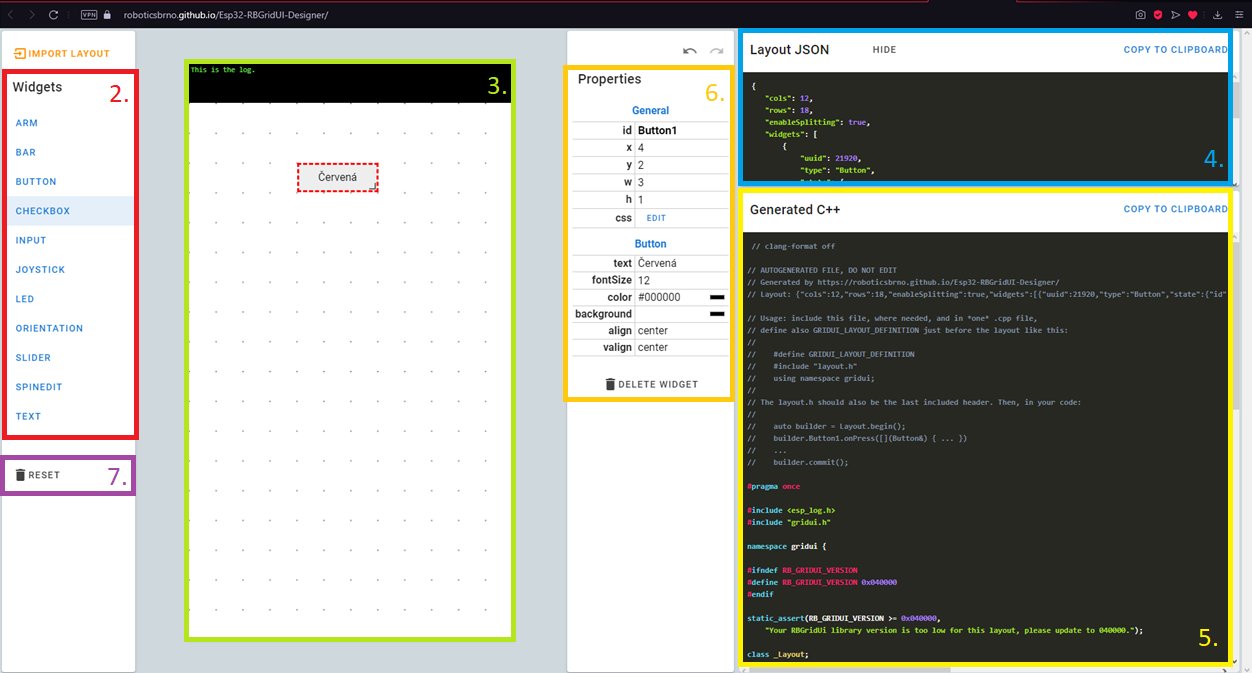
\includegraphics[width=1\textwidth]{img/Esp32-RBGridUI-Designer - malování.png}
	\caption{Prostředí stránky}
	%	\label{fig:install-sdk-3}
\end{figure}

\begin{enumerate}
	\item Postraní lišta, pri kliknutí na jakoukoliv komponentu, je uživatel schopen danou kamponentu přetáhnout na manipulační plochu
	\item Manipulační plocha, přetahují se sem tlačítka a nastavuje se jejich poloha a umístění, určuje vzhled řídící plochy v mobilu po stáhnutí aplikace
	\item Soubor, který je potřeba stáhnout a nahrát do stejné složky jako máme {/bf program}, nese informace toho, jakým způsobem jsme nanesli komponenty na manipulační plochu.
	\item {/bf Něco} %todo vysvětlit
	\item Bližší specifikace, určující umístění, barvu, a název tlačítka, které bylo vytvořeno na manipulační ploše. 
	\item Tlačítko Reset které vymaže veškeré komponenty z Manipulační plochy
\end{enumerate}


{\em Esp32-RBGridUI-Designer} je propojený s aplikací RBControler, %todo odkaz no google play + reference

\section{Vytvoření tlačítek}
Teď přišel čas na to, abych si připravila vlastní tlačítka. Každé tlačítko zpustí jiný mód, a ještě jsem tam chtěla mít tlačítko na vypnutí, takže jsem si celkově nadefinovala 5 tlačítek a pojmenovala je tak, abych se v jejich barvách vyznala. A poté jsem klikla na tlačítko copy to clipboad a zkopírovala jsem celý layout to textového souboru do stejné složky, jako jsem měla nový program  


\begin{figure}[htbp]
	\centering
	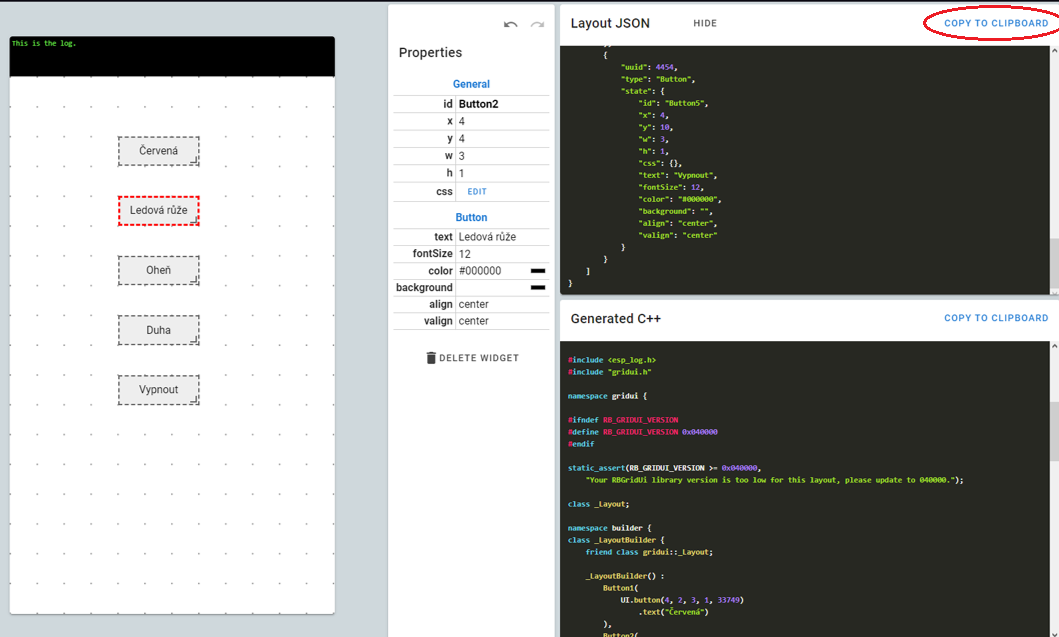
\includegraphics[width=0.8\textwidth]{img/Esp32-RBGridUI-Designer - Tlačítka.png}
	\caption{Tlačítka}
	%	\label{fig:install-sdk-3}
\end{figure}

\section{Nový program} %todo Předělat celý tento odstavec
%todo Vyřešit/předělat nahrání programů?
Pro to, aby Ledky byli kompatibilní s programem, jsem si musela upravit jeden program který jsem dostala a který mi na mobilu fungoval. % todo odkaz na github 
Funkce void Setup() v následujícím programu ukazuje část nastavení mobilu a pak definování tlačítek a jejich funkcí. Funkce void Loop() dokončuje ukázku definování tlačítek, která je provedená pomocí funkce switch
%todo Reference na kapitolu
Odkaz na Github

\lstinputlisting{Code/new-program - Setup.cpp}

\lstinputlisting{Code/new-program - Loop.cpp}

\section{Propojení mobilu a ESP32-DevkitC a kontrola funkčnosti}
První krok byl, že jsem si stáhla aplikaci z Google play jménem RB Controler %todo odkaz
Poté jsem zapojila ESP32-DevkitC, ověřila jsem si, že je v něm nahraný konečný program a připojila jsem se na wifinu jménem LEDLED. 

%todo Zde bude screenshot obrazovky mého mobilu.

Teď už jenom chtělo vyzkoušet, jak moc je daný program kompatibilní a funkční. %todo odkaz na video?

\newpage
